Let $X \in \cbrak{i}_{i=1}^{6}$ and $f_i$ be the correspnding frequency.  Then, 
\begin{align}
\pr{X=i} &= \frac{f_i}{1000}
\end{align}
and
\begin{align} 
\pr{X=6} &= \frac{14}{200}
\\
&= 0.07
\end{align}
The related code is available in 
\begin{lstlisting}
solutions/1-10/codes/probexm/probexm4.py
\end{lstlisting}
%\begin{figure}[!ht]
%	\centering
%	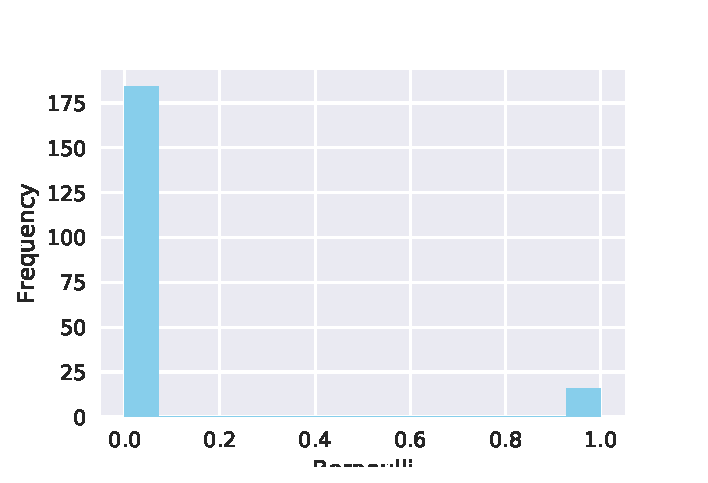
\includegraphics[width=\columnwidth]{./figures/probexm/probexm4.eps}
%	\caption{bernoulli distribution of no to be 6}
%	\label{fig:bt2}
%	\begin{lstlisting}
%	figs/probexm/probexm4.eps
%	\end{lstlisting}
%\end{figure}
